Et notchfilter er et spesialtilfelle av båndstop hvor Q-Verdien er veldig høy.
Signalet sender til både et lavpass- og et høypassfilter før de legges sammen
i en adder som plusser sammen signalene.

\begin{figure}[H]
  \caption{Skjematikk for notch filter}
  \centering
  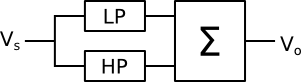
\includegraphics[width=0.67\textwidth]{./img/notch-kobling}
\end{figure}

Den resulterende formen på signalet blir

\begin{figure}[H]
  \caption{Notch filter frekvens og forsterkning}
  \centering
  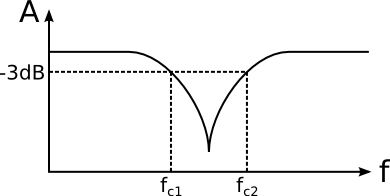
\includegraphics[width=0.67\textwidth]{./img/notch-frekvens}
\end{figure}
